\begin{singlespacing}
\chapter{A search for new phenomena}
\label{chapter:2ljets}
%
\begin{epigraphs}
\qitem{%
An experiment is never a failure solely because it fails to
achieve predicted results. An experiment is a failure only when it also
fails adequately to test the hypothesis in question, when the data it
produces don’t prove anything one way or another.%
}%
{Robert M. Pirsig~\cite{pirsig1999zen}}
\qitem{%
But there is one feature I notice that is generally missing in cargo cult
science. \ldots\
% That is the idea that we all hope you have learned in studying science in
% school--we never say explicitly what this is, but just hope that you catch
% on by all the examples of scientific investigation. It is interesting,
% therefore, to bring it out now and speak of it explicitly.
It's a kind of scientific integrity, a principle of scientific thought that
corresponds to a kind of utter honesty --- a kind of leaning over backwards.%
}%
{Richard Feynman~\cite{feynman1974cargo}}
\end{epigraphs}
\end{singlespacing}


% begin with physics content and results

Our central result is Figure~\ref{fig:2ljets_summary}, which shows the names,
data, and fitted background expectations with error bars in all main regions.
This figure illustrates the background part of a \clown{likelihood}
which is extended with signals to test alternative models.
Exclusion contours testing the addition of C1N2 and GMSB signals to these
backgrounds are shown in Figures~\ref{fig:2ljets_contours_c1n2}
and~\ref{fig:2ljets_contours_gmsb}.
Interpretations of discovery region data are displayed in
Table~\ref{tab:2ljets_discovery}.


% summary plot

\begin{figure}[tp]
\centering
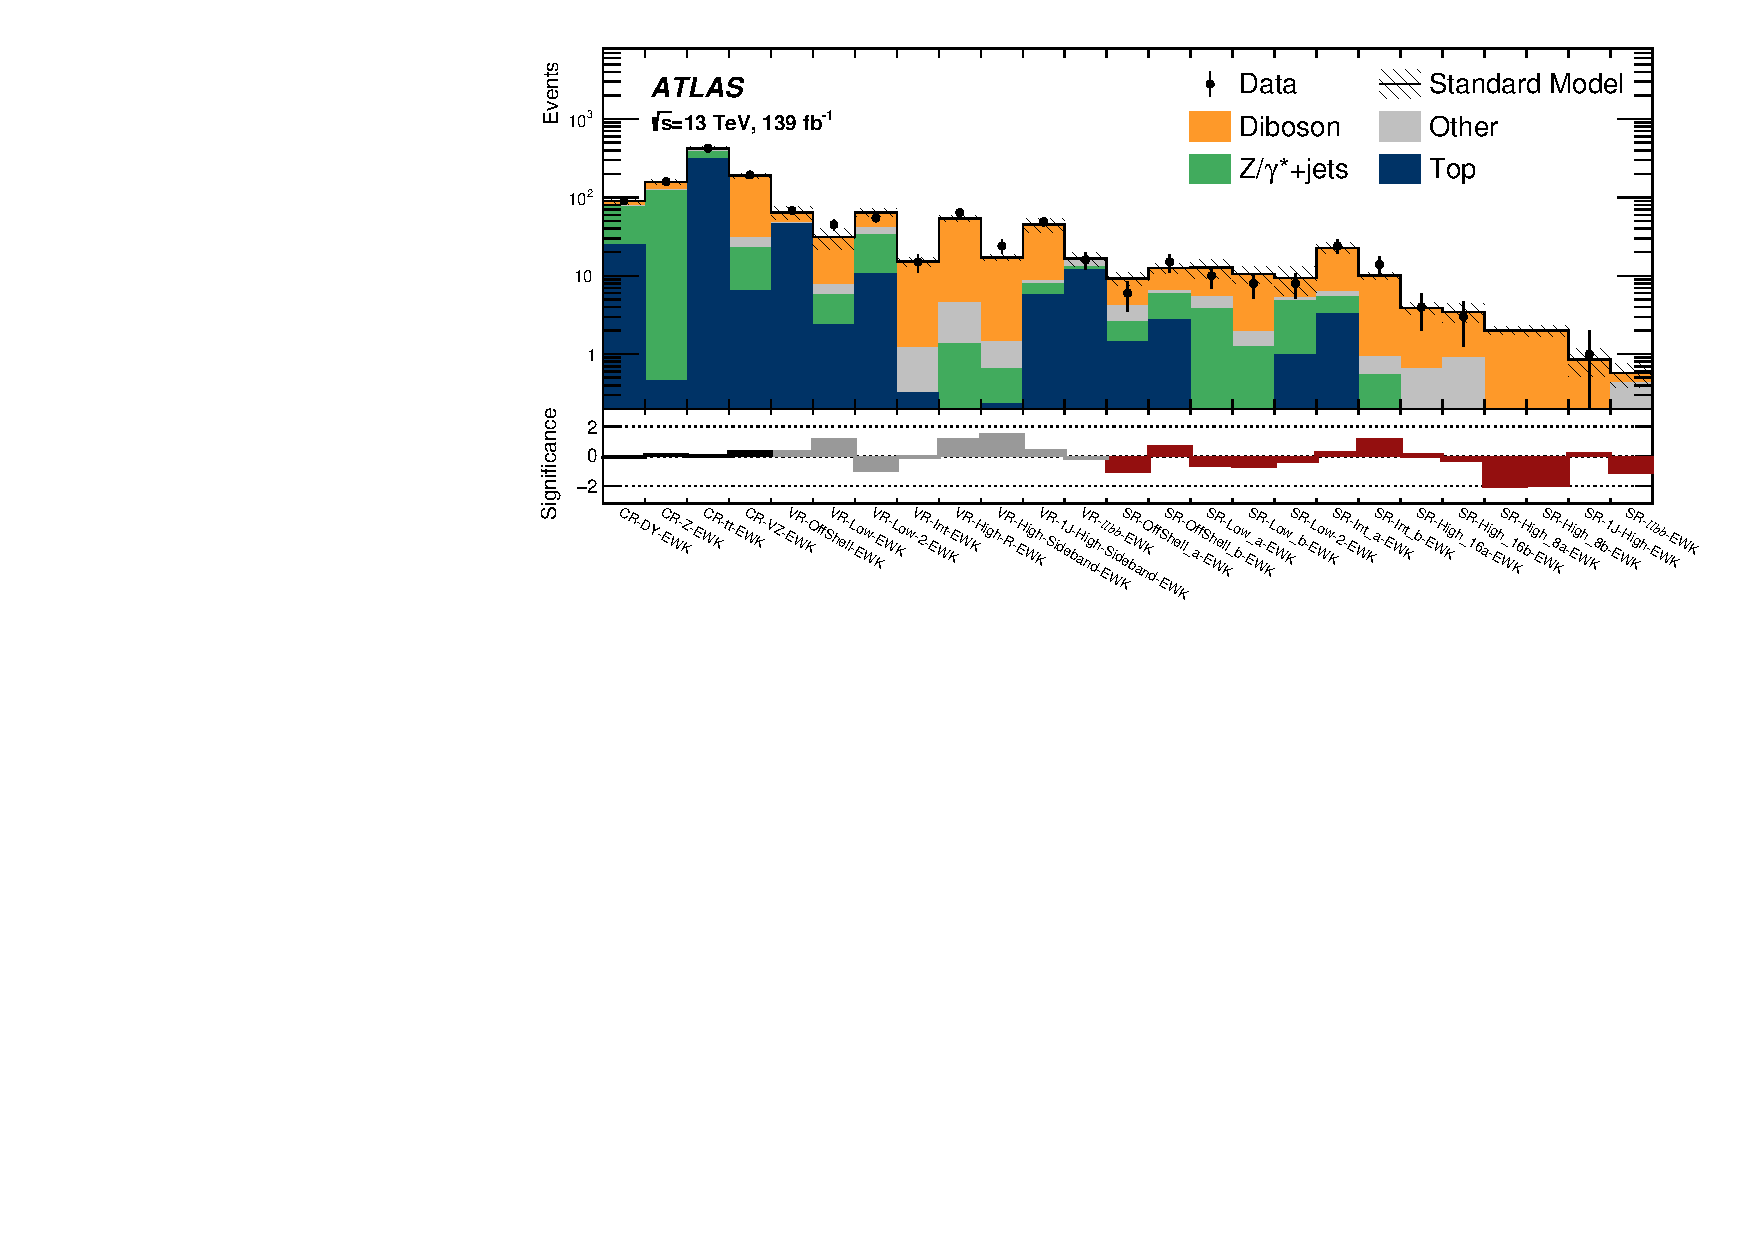
\includegraphics[width=\textwidth]{figures/2ljets_summary_log.pdf}
\caption{%
Data of the $\twoljets$ electroweak analysis with \emph{post-fit} backgrounds
for which the lower panel shows $S_\mathrm{ATLAS}$ from
Equation~\ref{eqn:significance_atlas}.
Control, validation and signal regions are shown from left to right, with the
regions within each category ordered approximately by their typical $\ptmiss$.
Likelihoods from validation regions are not included in the fit.
The `Top' category contains $t\bar t$ and $tW$ processes, and
`Other' contains fake/non-prompt lepton, higgs, triboson, $t\bar tZ$, and other
rare top processes.%
}
\label{fig:2ljets_summary}
\end{figure}


% TODO signal region plots here


\begin{figure}[t]
\centering
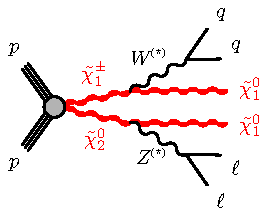
\includegraphics[width=0.48\textwidth]{figures/2ljets_c1n2_llqqn1n1_wz.pdf}
\quad
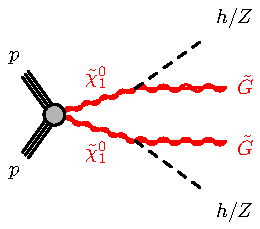
\includegraphics[width=0.45\textwidth]{figures/2ljets_n1n1_hhggzz.pdf}
\caption{%
Supersymmetric signal processes in the $\twoljets$ electroweak analysis.
\\[0.5em]
Left: C1N2, where the initial $\chargino{1}\textrm{--}\neutralino{2}$ pair
is produced through a $s$-channel $W^{\pm}$ resonance and the masses of
weak bosons in decays are bounded by the mass splitting
$m(\chargino{1}, \neutralino{2}) - m(\neutralino{1})$.
We explore the parameters
$m(\chargino{1}, \neutralino{2})$ and $m(\neutralino{1})$.
\\[0.5em]
Right: GMSB, where the initial $\neutralino{1}\textrm{--}\neutralino{1}$ pair
is produced by soft decays from pairs including $\chargino{1}$,
$\neutralino{2}$ or $\neutralino{1}$.
Although the $h$ and $Z$ bosons decay to many states, we target
$Z\rightarrow \ell\ell$ with
$h/Z\rightarrow bb/jj$.
We explore the parameters
$m(\neutralino{1})$ and $B(\neutralino{1} \rightarrow h \tilde{G})$ with fixed
$m(\chargino{1}, \neutralino{2}) - m(\neutralino{1}) = 1~\eV[G]$.
}
\label{fig:2ljets_summary}
\end{figure}




% exclusion plots

\begin{figure}[tp]
\centering
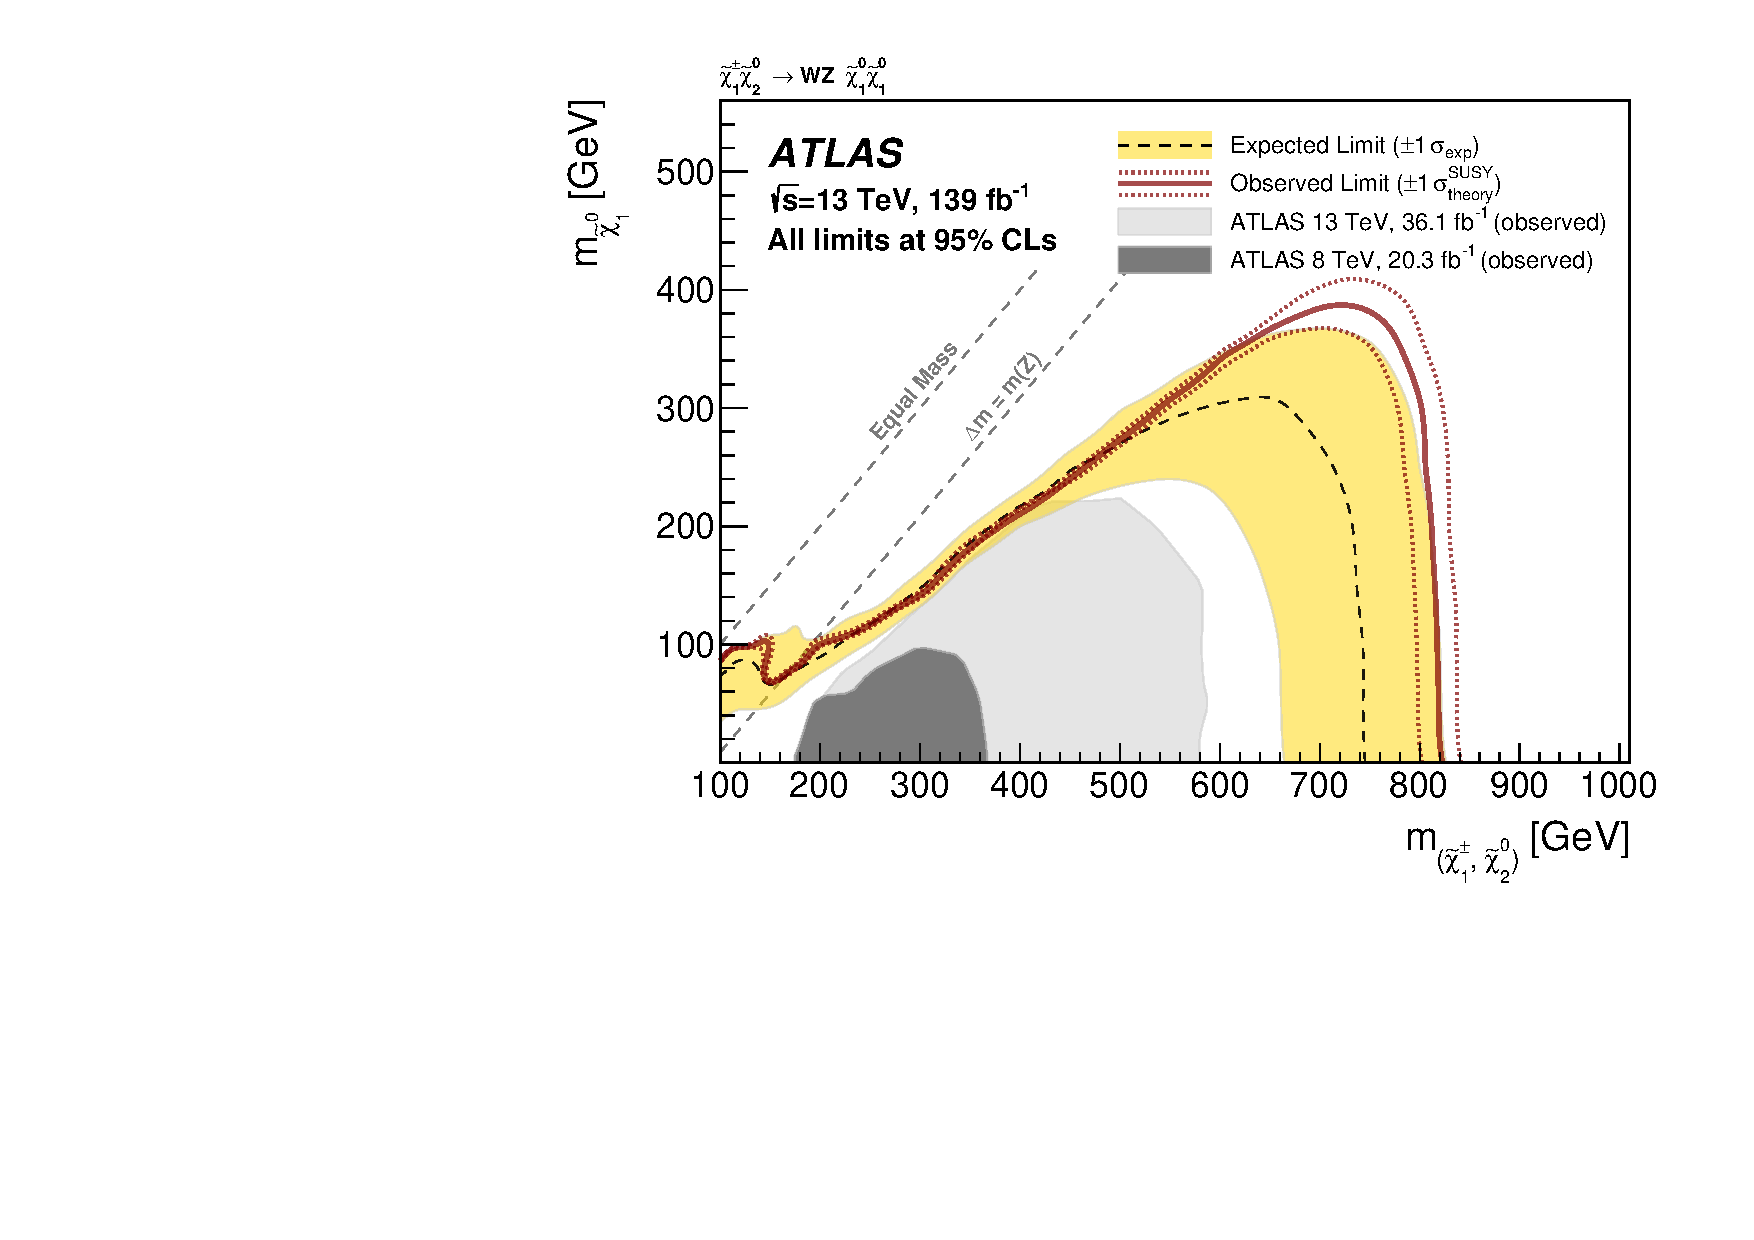
\includegraphics[width=0.99\textwidth]{figures/2ljets_contours_c1n2.pdf}
\caption{%
Contours for the C1N2 model in the $\twoljets$ electroweak analysis.
Space below the solid red line is labelled as excluded and its dotted
neighbours show the result if all signal cross-sections are varied up and down
by theoretical error bars.
The yellow band shows the $\pm1$-sigma region of exclusion contours
from asymptotic approximations to the prior distribution of the test statistic.
Grey areas are observed limits from the two-lepton parts
of~\cite{SUSY-2016-24} and~\cite{SUSY-2013-11}.
Exclusion is defined by the $95\%$ $\mathrm{CLs}$ prescription
in asymptotic approximations.
All contours are interpolated from a sparse grid.
}
\label{fig:2ljets_contours_c1n2}
\end{figure}

\begin{figure}[tp]
\centering
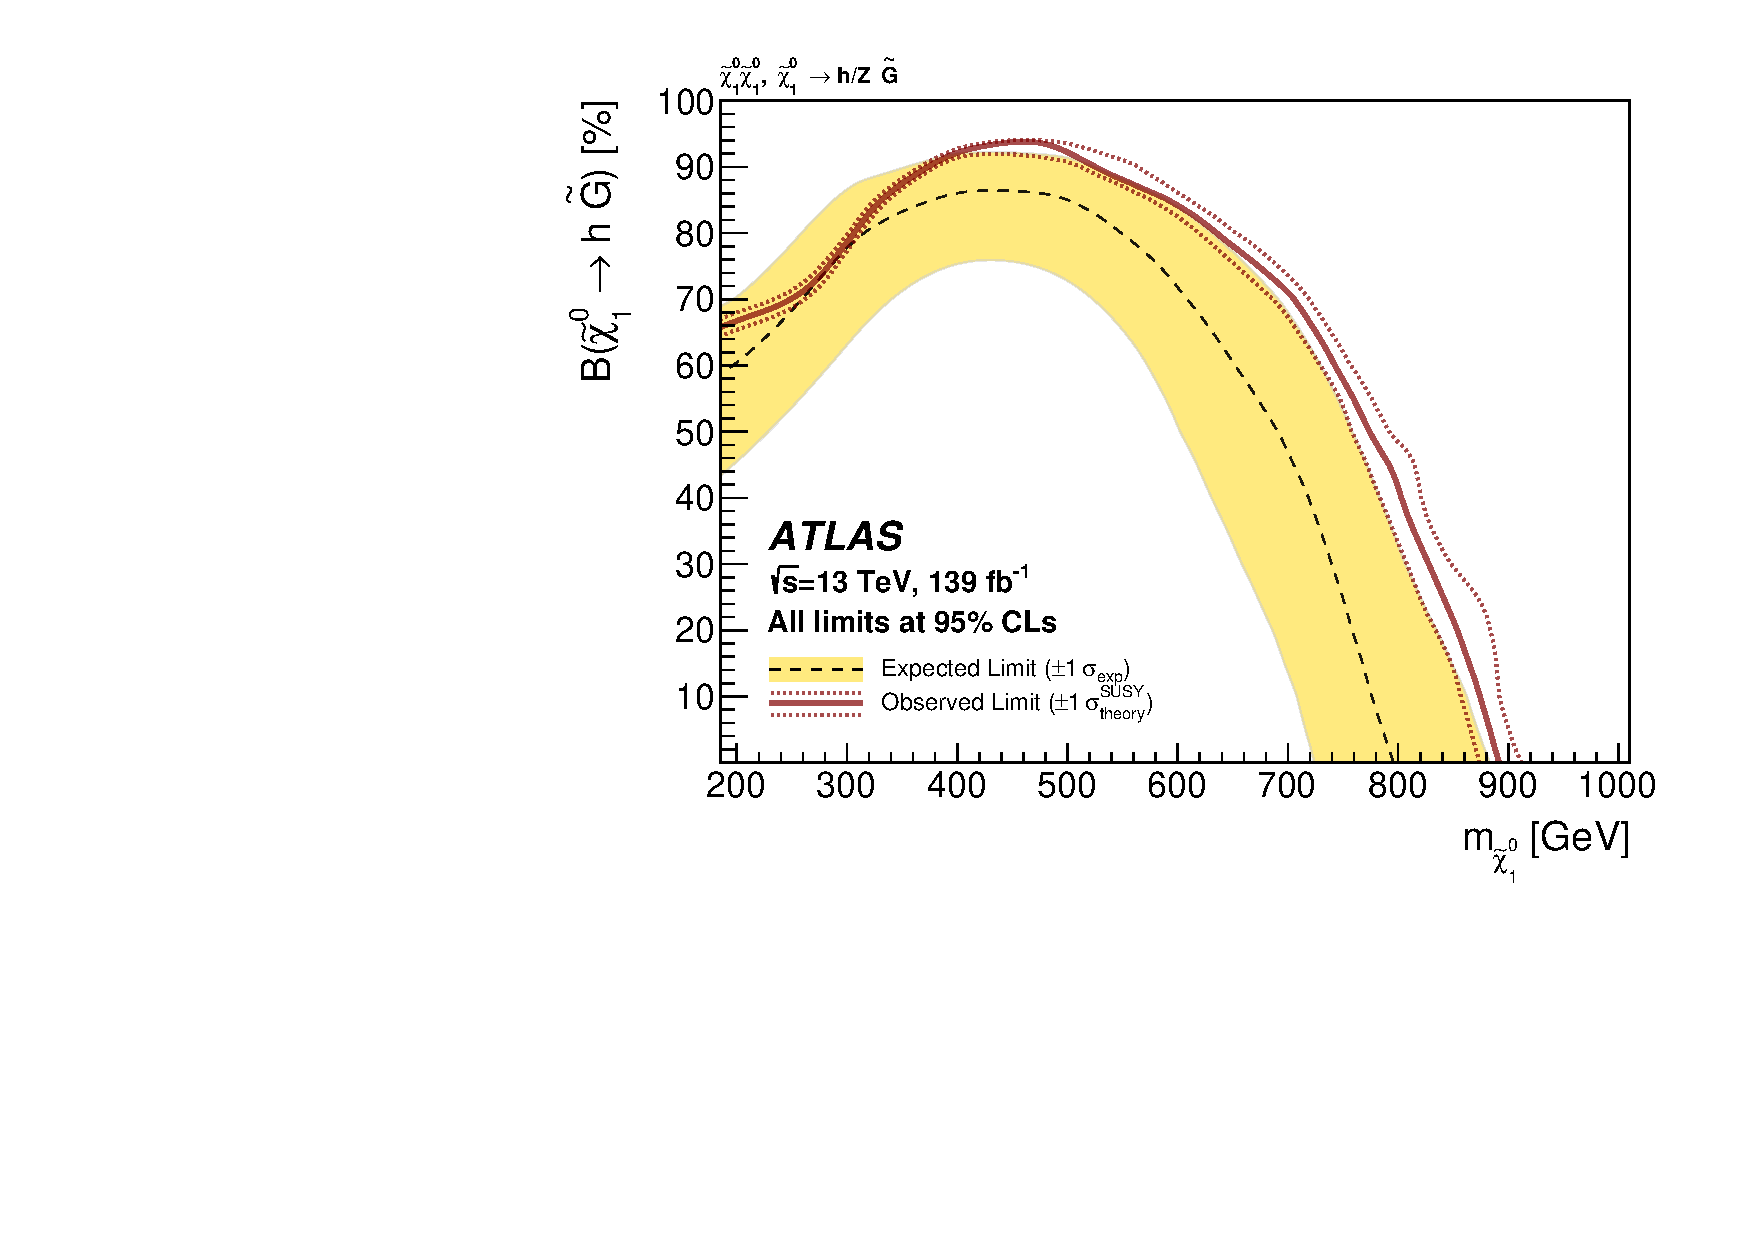
\includegraphics[width=0.99\textwidth]{figures/2ljets_contours_gmsb.pdf}
\caption{%
Contours for the GMSB model in the $\twoljets$ electroweak analysis.
Space below the solid red line is labelled as excluded and its dotted
neighbours show the result if all signal cross-sections are varied up and down
by theoretical error bars.
The yellow band shows the $\pm1$-sigma region of exclusion contours
from asymptotic approximations to the prior distribution of the test statistic.
Exclusion is defined by the $95\%$ $\mathrm{CLs}$ prescription
in asymptotic approximations.
All contours are interpolated from a sparse grid.
}
\label{fig:2ljets_contours_gmsb}
\end{figure}


% upper limits
% definitely want this after pictures
\FloatBarrier
\begin{table}[tp]
\centering
\begin{tabular*}{\textwidth}{lccccccc}
{Region} &
\multicolumn{1}{c}{Fitted} &
\multicolumn{1}{l}{Data} &
$\langle A\epsilon{ \sigma}\rangle_{\mathrm{obs}}^{95}~\mathrm{fb}$ &
\multicolumn{1}{c}{$S_{\mathrm{obs}}^{95}$}  &
\multicolumn{1}{c}{$S_{\mathrm{exp}}^{95}$} &
$\mathrm{CLb}$ &
$p(s=0)$  \\[1.5ex]
DR-OffShell      & $22.1\pm2.7$ & 21 & $0.10$ & $14.3$ & $12.3^{+4.7}_{-3.1}$ & $0.68$ & $0.50$ \\[.5ex]
DR-Low           & $22\pm4$ & 18 & $0.08$ & $10.8$ & $15.3^{+5.7}_{-4.0}$ & $0.09$ & $0.50$ \\[.5ex]
DR-Int           & $35\pm4$ & 38 & $0.15$ & $20.9$ & $17.5^{+5.9}_{-3.9}$ & $0.73$ & $0.23$ \\[.5ex]
DR-High          & $3.9\pm0.5$  & 0  & $0.02$ & $3.0$ & $5.6^{+2.2}_{-1.5}$ & $0.00$ & $0.50$ \\[.5ex]
DR-$\ell\ell bb$ & $0.51\pm0.20$  & 0  & $0.02$ & $3.0$ & $3.0^{+1.3}_{-0.0}$ & $0.19$ & $0.50$ \\[.5ex]
\end{tabular*}
\caption{%
Upper limit results in discovery region.
The fitted yield is in the background-only model constrained by the data in each region.
Limits are intended to reflect constrains on additive signal contributions.
\\[0.5em]
Left to right:
the region name,
the post-fit background expectation,
the number of data observed,
the observed $95\%$ $\mathrm{CLs}$ upper limit on the visible cross-section
$\langle\epsilon\sigma\rangle_\mathrm{obs}^{95}$,
its corresponding signal expectation $S_\mathrm{obs}^{95}$,
the \clown{expected} $95\%$ upper limits on the signal expectation $S_\mathrm{exp}^{95}$
as would be obtained were the test statistic given by its central or
$\pm1$-sigma variations,
$\mathrm{CLb}$ evaluated with the signal expectation set to the observed upper limit,
and the discovery $p$-value (capped at $0.5$) with its equivalent significance.
\\[0.5em]
Upper limits use the one-sided profile likelihood test statistic.
The discovery $p$-value uses a profile likelihood test statistic in a one-sided test.
All $p$-values are estimated by simulation of alternative data.
\TODO{add labels and references to asymptotic formulae paper}
}
\label{tab:2ljets_discovery}
\end{table}


\paragraph{My contributions}
\begin{itemize}
\item Design, implementation and execution of the electroweak part of the analysis.
\item Analysis Contact from January to October 2020.
\item Production of main data inputs for all three analyses
and the RJR $3\ell$ search \TODO{cite}.
I produced all systematic variations for the background samples and all
electroweak signal samples.
Other group members assisted with the central background sample.
\item Integration with ATLAS combinations and pMSSM scan efforts by
performing their validation studies and serializing the analysis results.
\item Preparation of electroweak results for publication in the paper, and the
public HEPData record~\cite{maguire2017hepdata}.
\end{itemize}

\section{Context}
% previous results on 2(/3)L from ATLAS
% other constraints on these models from ATLAS/CMS
% previous region design, motivation for this work

\section{Design}

% CRs go in with relevant SR category
\subsection{High}

\subsection{Intermediate}

\subsection{Low}

\subsection{Off-shell}

\subsection{Discovery}

\section{Modelling}
% backgorund samples
% matrix method fakes

\subsection{Fake/non-prompt leptons}

\section{Validation}

\section{Systematics}

\section{Results}


